\section{3D model reconstruction of cloth} \label{section:3dclothrecon}

\subsection{Overview} 

For 3D human body model, we use Skinned Multi-Person Linear model (SMPL)\cite{Loper2015SMPLAS}, because SMPL has well defined control variables for shape and pose, and well defined parameter estimation algorithms as well. For similar reasons, SMPL\cite{Loper2015SMPLAS} model have been utilized in many research works \cite{Zanfir2018HumanAT,Weng2018PhotoW3}. Furthermore, since it is based on blend skinning, SMPL is compatible with existing rendering engines\cite{Loper2015SMPLAS} and made available for research purposes. SMPL is a skinned vertex-based model that accurately represents a wide variety of body shapes in natural human poses. The parameters of the model are learned from data including the rest pose template, blend weights, pose-dependent blend shapes, identity-dependent blend shapes, and a regressor from vertices to joint locations. Unlike previous models, the pose-dependent blend shapes are a linear function of the elements of the pose rotation matrices. This simple formulation enables training the entire model from a relatively large number of aligned 3D meshes of different people in different poses. \cite{Loper2015SMPLAS} 


\begin{figure}[t]
\centering
% 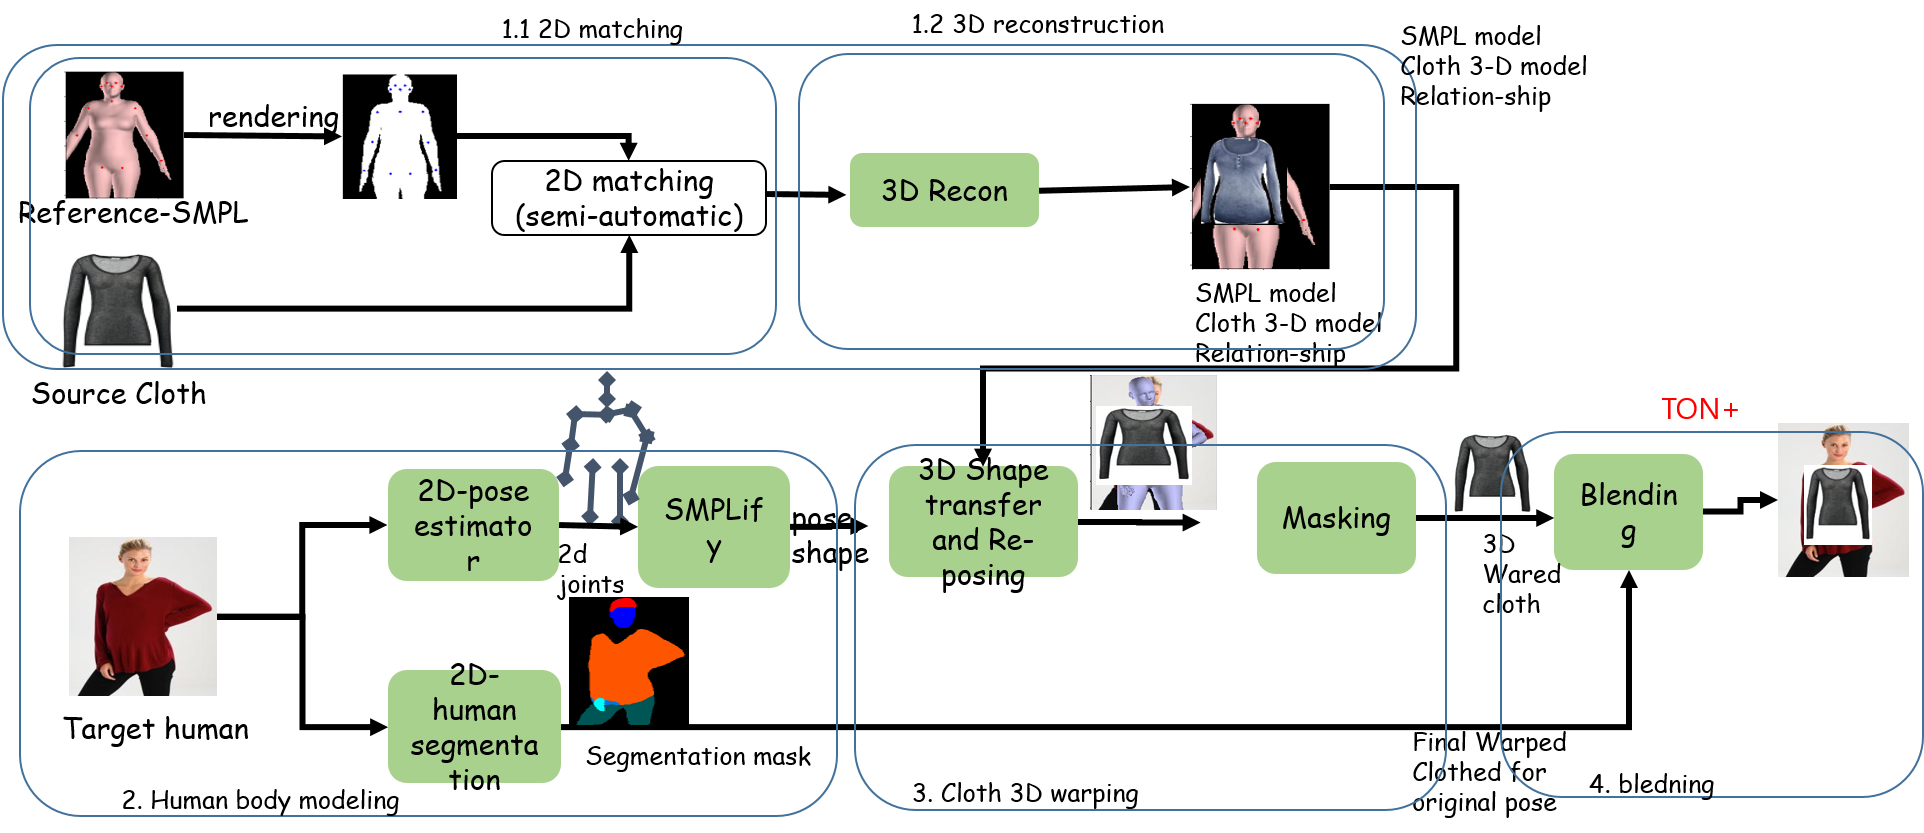
\includegraphics[height=4.5cm, scale=1]{figures/pipeline.png}   % TODO
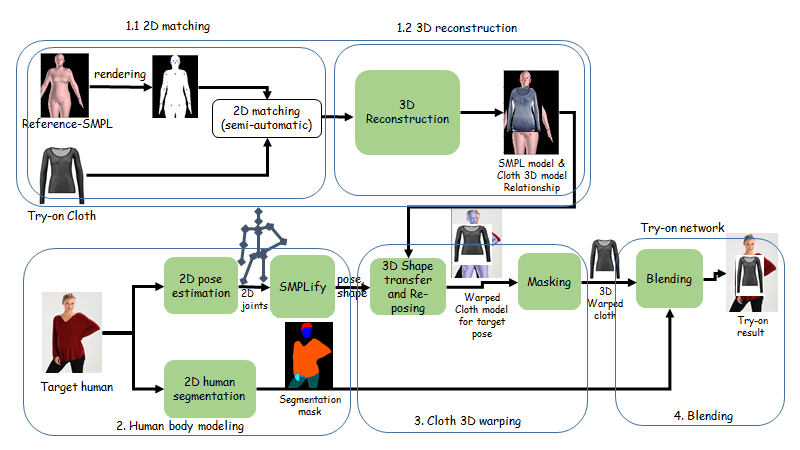
\includegraphics[scale=0.6]{figures/updatedpipeline.png}
\caption{Proposed pipeline}
\label{fig:pipeline}
\end{figure}


For estimating the SMPL\cite{Loper2015SMPLAS} parameters, we use SMPLify\cite{Bogo2016SMPLify} method in this study. However, any other methods can be used since we assume nothing on the procedure and use estimated parameters only. SMPLify\cite{Bogo2016SMPLify} uses 2D human body joint information often obtained from deep learning based method like DeepCut\cite{pishchulin2016deepcut} or OpenPose\cite{Cao2018OpenPoseRM}, and minimize the projected joint locations and the given (considered true) 2D joint locations. The cost function can include other priors and silhouette information. We made minor optimization for half body dataset, such as joint location mapping between the joints of used fashion data set and SMPLify joint definition, and conditional inclusion of invisible joints and initialization step.  From our experiments with all 2032 test images, we found that the SMPLify quality should be much improved for fully automatic application to VTON application. So the result included in this paper excluded the bad matching cases which is around 30\% of all test images.    
  
Clothed human reconstruction using 3D SMPL model\cite{Loper2015SMPLAS} have been studied in several previous works \cite{Weng2018PhotoW3,Zanfir2018HumanAT}. Although we are successful in modeling human body, there are further difficulties to recover the clothed human model from body model. It is due to the cloth vertices, which do not directly correspond to the human body's. Even if it does, it is still difficult to estimate the differences between two. Also, the textures of clothes can be occluded by other parts of clothes and human body parts. Previous works try to solve the problem in the given image condition. Therefore, the results are strongly dependent upon the input images. In this paper, we make this step easy by using simple standard human pose, where all frontal parts of clothes are well separated and visible. This setup cannot handle all problems in the clothed human model reconstruction, however, it can greatly make it easy. The following subsection describe the procedure in details.



\subsection{2D Standard Cloth matching}


To align the try-on cloth image with 3D SMPL\cite{Loper2015SMPLAS} body model, first their dimension spaces should be matched. Natural way would be first rendering the SMPL\cite{Loper2015SMPLAS} body model into 2D image space. However, as stated above, the matching between cloth image and body silhouette is not a simple task. For simplicity, we assume we can segment the silhouette, so that the remaining area can be easily matched by Shape-Context Matching (SCM)\cite{BelongieMP02} algorithm. We argue that, for virtual try-on commercial application, this step can be monitored by service provider side which is practically acceptable. The manual operation from the customer in the try-on step would not be acceptable in general service environment.   

\begin{equation}
(I_{c, warped}, M_{c, warped})  = T_{SMPL} ((I_c, M_c))
\end{equation}


\begin{figure}
\centering
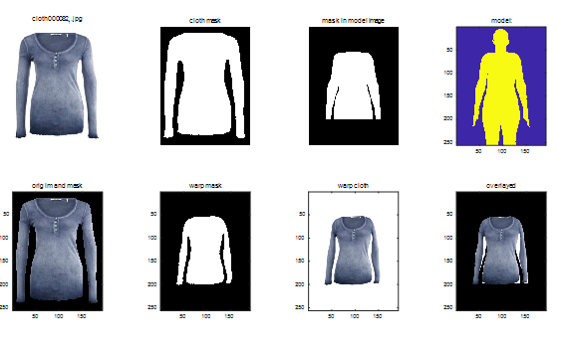
\includegraphics[width=9cm]{figures/2dmatching.png}   % TODO
\caption{2D matching between clothing image and 3D body model silhouette mask}
\label{fig:2DmatchingOfClothAndBody}
\end{figure}


\subsection{3D cloth model reconstruction }


The 3D reconstruction process from aligned cloth image and projected silhouette consists of 2 steps. First, the vertices of 3D body mesh are projected into 2D image space, the boundary vertices in 2D spaces, and the cloth boundaries are used for corresponding points. The corresponding points in the cloth boundary is defined as the closest points from the projected vertices. This step works well in our cases differently from Photo Wake-up\cite{Weng2018PhotoW3} study, because the part of body and cloth are not self-overlapped. This is a implementation benefits of our approach. From the corresponding point pairs, a This-Plate Spline (TPS)\cite{Bookstein1989PrincipalWT} parameters are estimated and applied to the mesh points. The new mesh points are considered as the vertices projected from 3D mesh of cloth. From 2D points to 3D points are done with inverse projection with depth obtained from the body with a small constant gap. In reality the gap between the cloth and body cannot be constant but it works with tight or simple clothes. Further research works are needed for accurate depth estimation.   


\begin{equation}
V_{clothed} = Pjt^{-1} ( T( (Pjt(V_{body})), depth(V_{body}) )
\end{equation}


The try-on cloth images are used as the texture for the 3D cloth mesh. We can filter the vertices corresponding to cloth and get the cloth 3D mesh model. Figure \ref{fig:3DreconstructedCloth} shows the reconstructed cloth examples. 


\begin{figure}[t]
\centering
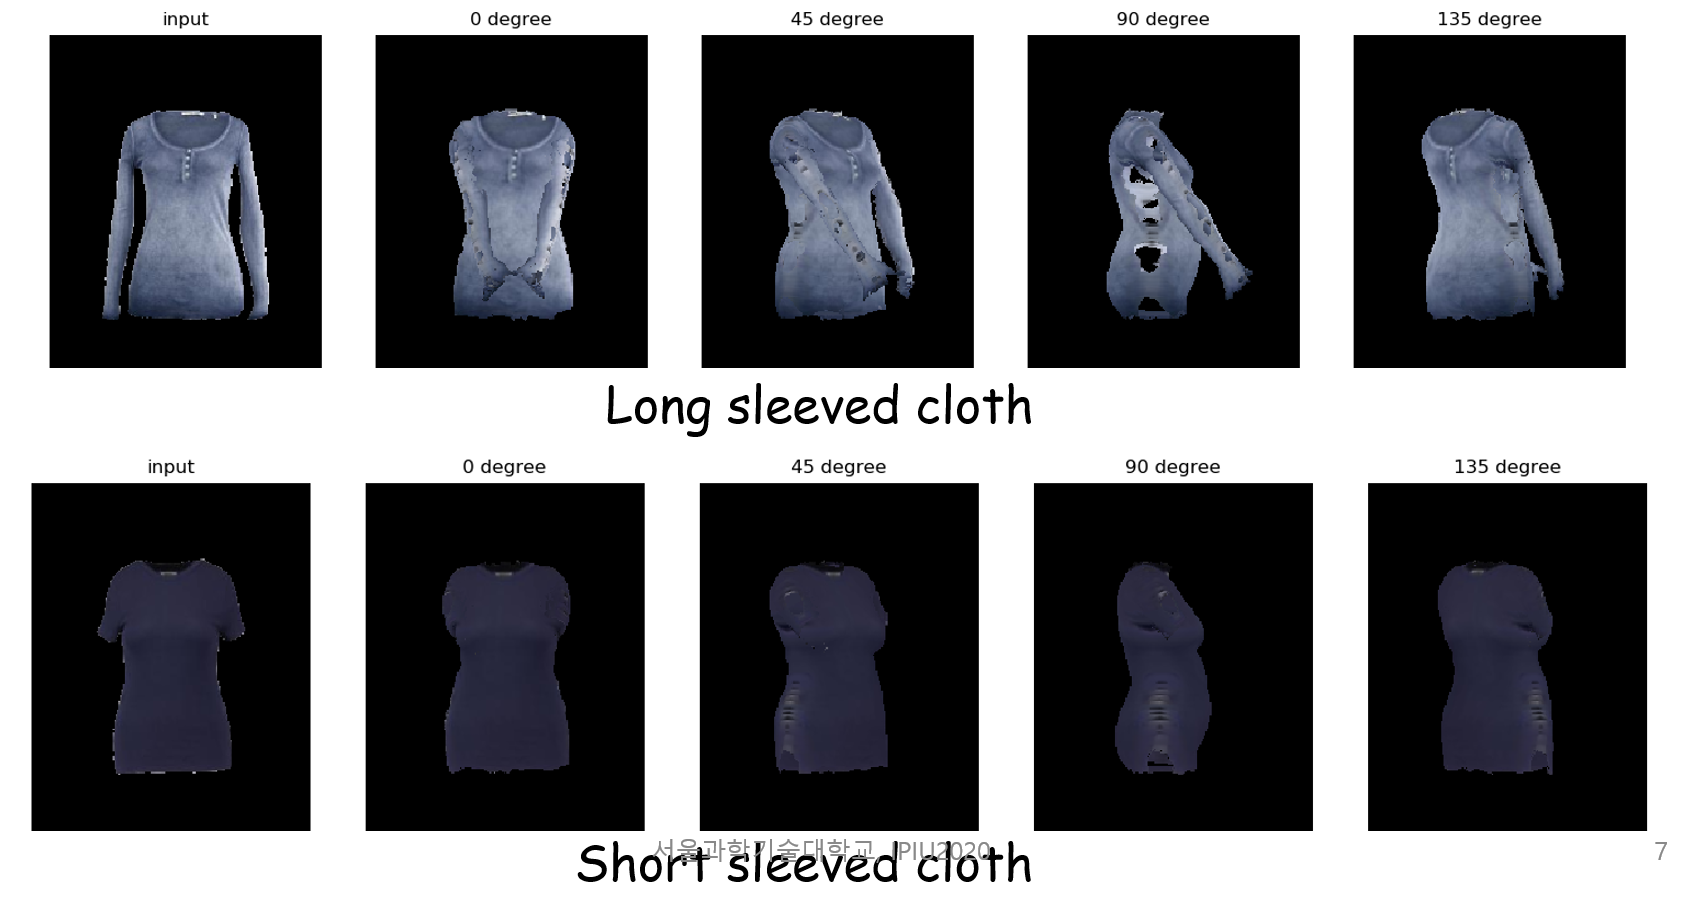
\includegraphics[height=6.5cm]{figures/3dclothrecon.png}   % TODO
\caption{3D reconstructed cloth}
\label{fig:3DreconstructedCloth}
\end{figure}



